\section{Logická funkce, její vyjádření pomocí tabulky, algebraického výrazu a map. Úplný součtový a součinový tvar algebraického vyjádření logické funkce. Metody a principy minimalizace logických funkcí. Úprava logické funkce pro realizaci pomocí členů NAND a NOR.}

\subsection{Logická funkce}
Matematický model logického kombinačního obvodu. \\
Jestliže hodnota výroku y závisí na hodnotách výroku \(x1, x2,..,xn\), pak říkáme, že logická proměnná y je logickou funkcí proměnných \(x_1,x_2,..,x_n\). Kde \(x_1,x_2,..,x_n\) je n-tice tvořená prvky 0 a 1.\\

Počet možných logických funkcí je \(2^n\), kde n je počet proměnných.

\begin{figure}[h!]
    \centering
    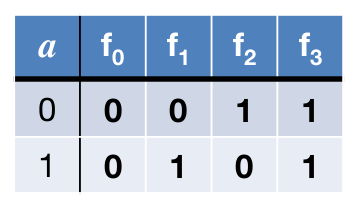
\includegraphics[scale = 0.5]{img/LogFce1.png}
    \caption*{Logická fce jedné proměnné}
\end{figure}

Úplně zadaná logická funkce, je taková funkce kde známe hodnotu pro všechny možné kombinace vstupních hodnot.\\
Neúplně zadaná logická funkce je taková, kde pro některé kombinace vstupních hodnot neznáme hodnota logické funkce. Pro neurčené stavy volíme hodnoty tak aby byla technická realizace co nejjednodušší.\\

\subsubsection{Vyjádření pravidvostní tabulkou}
Jednotlivé kombinace jsou uspořádány tak, jak roste binární číslo. Řádky tabulky značíme stavovými indexy s.
\begin{figure}
    \centering
    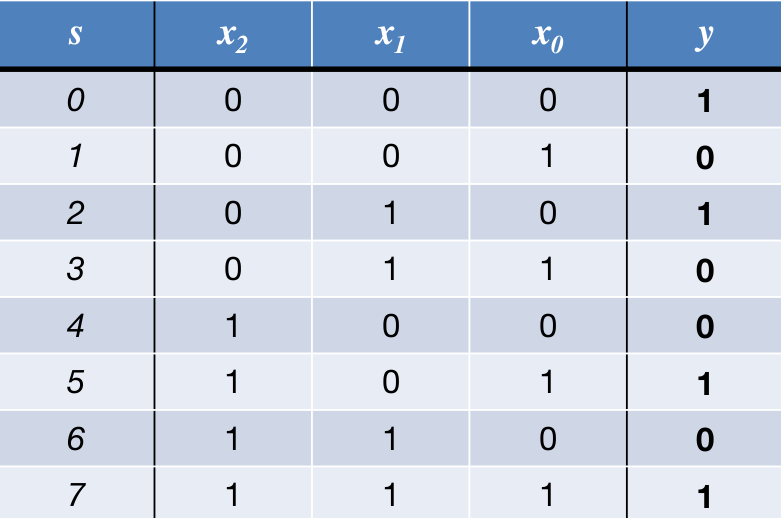
\includegraphics[scale = 0.4]{img/PravTabulka.png}
\end{figure}

\subsubsection{Vyjádření pomocí algebraického výrazu}
Logický výraz je tvořen logickými proměnnými a operátory.\\
Soustava operátorů musí být volena tak, aby umožnila vyjádřit libovolně složitou funkci. Tato soustava se nazývá úplný soubor logických funkcí. \\
Úplné soubory:
\begin{enumerate}
    \item AND, OR, NOT
    \item AND, XOR, XNOR
    \item Implikace, XOR
    \item Shefferova funkce(NAND)
    \item Piercova funkce(NOR)
\end{enumerate}

\subsubsection{Vyjádření pomocí map}
Karnaughovy mapy.\\
Uspořádány do čtverce nebo obdélníka. Každému poli jednoznačně odpovídá jedna kombinace vstupních proměnných. \\
Dovnitř do pole zapisujeme hodnotu výstupní proměnné.\\
Sousední pole jsou ta, která se dotýkají, pole na okrajích mapy(konce řádků, sloupců, rohy mapy), u mapy pro 5 a 6 proměnných pole symetrická podle os(vodorovné, svislé).\\
Sousední pole odpovídají mintermům či maxtermům, které se liší pouze v jedné hodnotě vstupní proměnné.\\
\subsubsection{Tvorba map}
Vzniká zrcadlením. \\
Při jednom vodorovném/svislém kroku mapou se změní vždy jedna hodnota vstupní proměnné(Grayův kód).\\
Názorná je do 4 proměnných. \\
\newpage
\begin{figure}[h!]
    \centering
    \begin{minipage}[b]{0.4\textwidth}
        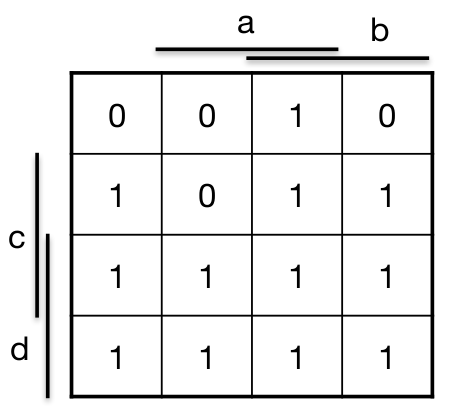
\includegraphics[width=\textwidth]{img/Mapa4.png}
    \end{minipage}
    \hfill
    \begin{minipage}[b]{0.4\textwidth}
        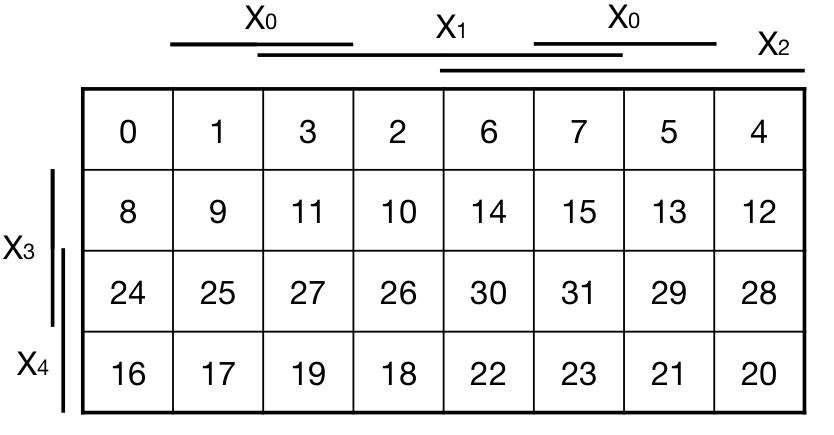
\includegraphics[width=\textwidth]{img/Mapa5.png}
    \end{minipage}
\end{figure}

\subsection{Úplný součtový a součinový tvar}
Term je výraz tvořený pouze proměnnými a operacemi AND(konjukce) nebo OR (disjunkce).\\
Minterm obsahuje všechny proměnné a pouze operaci AND.\\
Maxterm obsahuje všechny proměnné a pouze operaci OR.
\begin{center}
    Minterm: \(y = (x_2 \cdot \overline{x_1} \cdot x_0)\)\\
    Maxterm: \(y = (\overline{x_2} \cdot x_1 \cdot \overline{x_0})\)
\end{center}

Logickou funkci lze zapsat ve dvou základních tvarech.\\
\begin{itemize}
    \item Součtový tvar - úplná disjnukční normální forma. Součet mintermů, pro které funkce nabývá hodnotu 1.
    \item Součinový tvar - úplná konjunktní normální forma. Součin maxtermů, pro které funkce nabývá hodnotu 0.
\end{itemize}

\subsubsection{Součtový tvar - ÚDNF}
Součet elementárních logických funkcí, z nichž každá má hodnotu 1 pouze pro jeden řádek tabulky - takové funkce jsou mintermy.\\
V mintermu zapisujeme proměnné, které nabývají v příslušné kombinaci hodnoty 1 jako přímé a proměnné, které nabývají hodnoty 0 jako negované.\\
Minterm musí obsahovat všechny proměnné funkce.\\

\subsubsection{Součinový tvar - ÚKNF}
Součin elementárních logických funkcí, z nichž každá má hodnotu 0 pouze pro jeden řádek tabulky - takové funkce jsou maxtermy.\\
V maxtermu zapisujeme proměnné přesně naopak oproti mintermu.\\
Maxterm musí obsahovat všechny proměnné funkce.\\
\newpage
\begin{figure}
    \centering
    \includegraphics*[scale = 0.4]{img/Tvary.png}
\end{figure}
Rovnice pak jsou:
\begin{center}
    ÚDNF: \(y=\sum_{n = 1}(0,2,5,7)= \overline{x_2} \cdot \overline{x_1} \cdot \overline{x_0} + \overline{x_2} \cdot x_1 \cdot \overline{x_0} + x_2 \cdot \overline{x_1} \cdot x_0 + x_2 \cdot x_1 \cdot x_0 \)\\
    ÚKNF: \(y = \prod (1,3,4,6) = (x_2 \cdot x_1 \cdot \overline{x_0}) + (x_2 \cdot \overline{x_1} \cdot \overline{x_0}) + (\overline{x_2} \cdot x_1 \cdot x_0) + (\overline{x_2} \cdot \overline{x_1} \cdot x_0)\)
\end{center}
\subsection{Minimalizace logické funkce}
Vyjádření logické funce považujeme za minimální pokud má minimální počet termů, minimální počet nezávisle proměnných v každném termu, minimální počet negovaných proměnných.\\
Metody minimalizace jsou pomocí algebraických výrazů, pomocí map, speciálními metodami(např. metoda Quine-McCluskey).\\
\subsubsection{Minimalizace pomocí algebraických výrazů}
Pro součtový tvar to je spojování mintermů tak aby se vyloučily proměnné (\(a \cdot \overline{b} + b \cdot a = a(\overline{b} + b) = a\)). Vyloučením proměnných vznikají implikanty. Implikant považujeme za větší pokud pokrývá větší počet bodů funkce(tvořen menším počtem proměnných). Výsledkem je minimální disjunktní normální forma - MDNF.\\
Pro součinový tvar spojování maxtermů tak aby se vyloučily proměnné(\((a+b)\cdot(a+\overline{b}) = a + (b \cdot \overline{b}) = a\)).Vyloučením proměnných vznikají inhibenty. Výsledkem je minimální konjunktní normální forma. \\
Jak MDNF tak MKNF může mít jedna funkce více než jednu.

\subsubsection{Minimalizace Karnaughovy mapy}
Princip spočívá vpokrytí všech 1 (případně 0) soustavou smyček, přičemž:
\begin{itemize}
    \item Sousední pole se stejnou výstupní hodnotou lze spojovat do větších smyček.
    \item Smyčky musí být co největší, ale vždy obsahovat \(2^i\) polí.
    \item Smyček musí být co nejmenší počet
    \item Neurčené stavy nahrazujem čísly tak, abychom dostali co největší smyčky
\end{itemize}

\begin{figure}
    \centering
    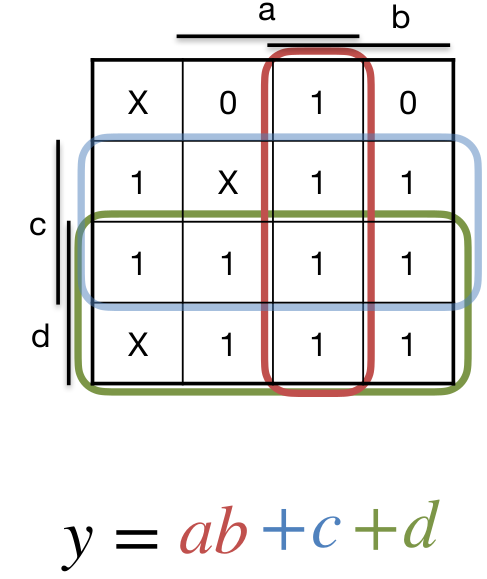
\includegraphics[scale = 0.3]{img/minMapa.png}
\end{figure}

\subsection{Úprava logické funkce pro realizaci pomocí NAND a NOR}
Pro nejjednodušší technickou realizaci je vhodné mít co nejmíň funkcí v úplném souboru. Existují 2 minimální soubory, NAND a NOR.
\subsubsection{Úprava na členy NAND}
Při úpravách na NAND vyjdeme ze součtové formy a použijeme DeMorganův zákon. \(\overline{a+b} = \overline{a} \cdot \overline{b}\)
Příklad úpravy na NAND:
\begin{center}
    \(\overline{x_1} \cdot \overline{x_0} + x_1 \cdot x_0 = \overline{\overline{\overline{x_1}\cdot\overline{x_0} + x_1 \cdot x_0}} = \overline{\overline{\overline{x_1}\cdot \overline{x_0}}\cdot\overline{x_1 \cdot x_0}}\)
\end{center}
\subsubsection{Úprava na členy NOR}
Při úpravách vycházíme ze součinové formy a použijeme DeMorganův zákon. \(\overline{a \cdot b} = \overline{a} + \overline{b}\)
Příklad úpravy na NOR:
\begin{center}
    \((\overline{x_1}+\overline{x_0})\cdot (x_1 + x_0) = \overline{\overline{(\overline{x_1}+\overline{x_0})\cdot (x_1 + x_0)}} = \overline{\overline{(\overline{x_1}+\overline{x_0})}+\overline{(x_1+x_0)}}\)
\end{center}

\section{Kombinační logické obvody: binární dekodér, multiplexor, demultiplexor, kodér, prioritní kodér, číslicový komparátor, binární sčítačka a odčítačka. Druhý doplněk. Logické obvody s třístavovým výstupem a s otevřeným kolektorem. Připojování zařízení na sběrnici.}
Kombinanční logický obvod je logický obvod, jehož hodnoty výstupních veličin jsou určeny pouze kombinací vstupních hodnot a nezávisí na předchozím stavu.

\subsection{Binární dekodér}
Převádí binární kód na kód 1 z N.\\
Pozice aktivního výstupu odpovídá binárnímu číslu přivedenému na vstupy dekokdéru.\\
Počet výstupů: N = \(2^k\), kde k je počet vstupů.\\
Mohou mít vstup Enable, který povoluje výstupy. Dokud není enable 1 tak jsou všechny výstupy 0.

\begin{figure}[h!]
    \centering
    \begin{minipage}[b]{0.4\textwidth}
        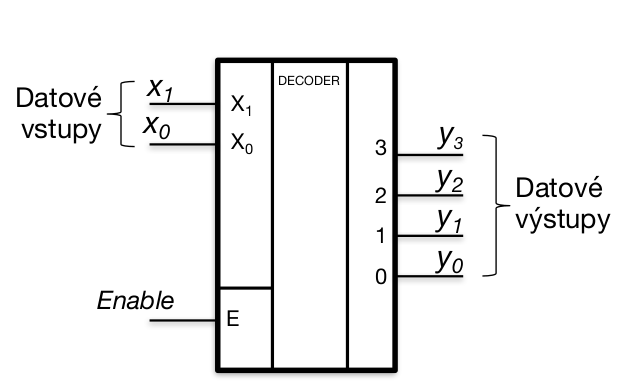
\includegraphics[width=\textwidth]{img/BinDekod.png}
    \end{minipage}
    \hfill
    \begin{minipage}[b]{0.4\textwidth}
        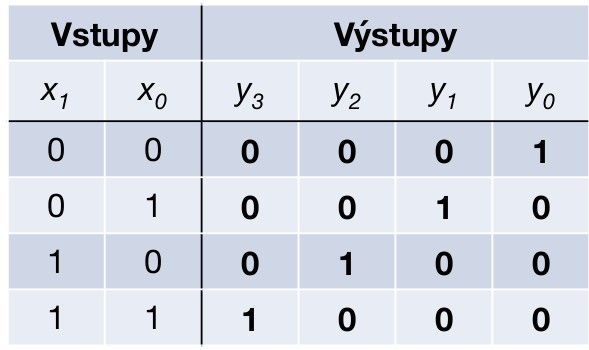
\includegraphics[width=\textwidth]{img/BinDekTab.png}
    \end{minipage}
\end{figure}

\subsection{Multiplexor}
Číslicový přepínač. Má dva druhy vstupů, adresové a datové. Jeden datový výstup.\\
Binární kód na adresových vstupech určuje číslo vstupu přivedené na výstup.\\
Počet takových vstupů: \(N = 2^k\), kde k je počet adresových vstupů.\\

\begin{figure}[h!]
    \centering
    \begin{minipage}[b]{0.4\textwidth}
        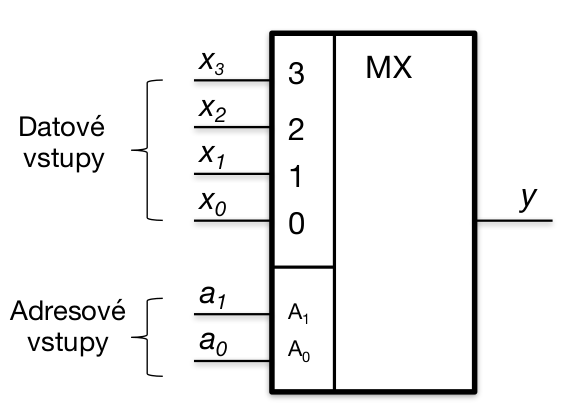
\includegraphics[width=\textwidth]{img/Multiplexor.png}
    \end{minipage}
    \hfill
    \begin{minipage}[b]{0.4\textwidth}
        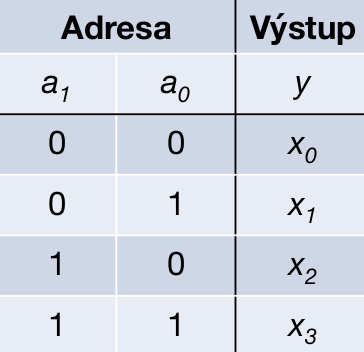
\includegraphics[scale = 0.3]{img/MultiTab.png}
    \end{minipage}
\end{figure}

\subsection{Skupinový multiplexor}
Přepíná skupiny signálů, také označován jako skupinový MX.\\

\begin{figure}[h!]
    \centering
    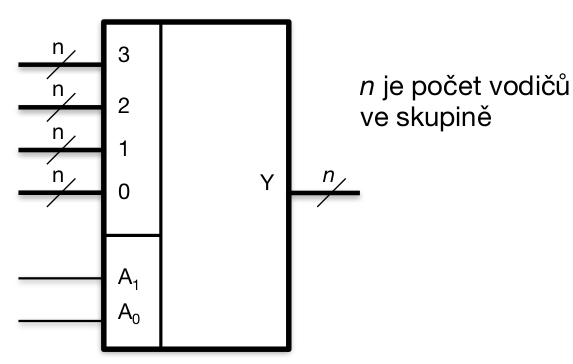
\includegraphics[scale = 0.3]{img/SkupMux.png}
\end{figure}

\subsection{Analogový a číslicový multiplexor}
Číslicový multiplexor umožňuje přenášet pouze binární signály, a to jednosměrně z vybraného vstupu na výstup. \\
Analogový multiplexor obsahuje přesné CMOS spínače, které umožňují obousměrný přenos analogových signálů. Pro výběr vstupů se používají opět binární adresovací vstupy.\\

\subsection{Demultiplexor}
Opak multiplexoru, binární kombinace adresových vstupů určuje na který výstup bude vstup propojen. \\
Obsahuje 1 datový vstup, N datových výstupů a k adresových vstupů, kde \(N = 2^k\).\\

\begin{figure}[h!]
    \centering
    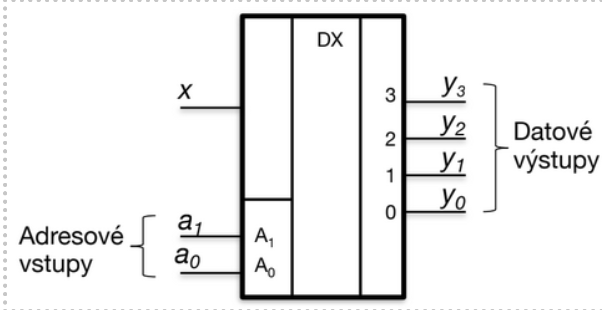
\includegraphics[scale = 0.3]{img/demux.png}
\end{figure}

\subsection{Kodér}
Opak dekodéru, převádí kód 1 z N na binární kód. \\
Je nutno zajistit aby byl vždy aktivní pouze jeden vstup. Toto je často těžko splnitelné proto se používá kodér prioritní.\\

\subsection{Prioritní enkodér}
Je přípustné aby byl aktivní více jak jeden vstup.\\
Vstupům přiřazena priorita. Nejjednodušší a nejčastější je odstupňování priority podle připojení, tedy priorita je pro každý vstup pevně stanovena (od nejmenšího indexu, nebo naopak).\\
Případ, kdy není aktivní ani jeden vstup, signalizuje pomocný výstup z. Při z = 0 nemají hodnoty na výstupech yi žádný význam.\\

\begin{figure}[h!]
    \centering
    \begin{minipage}[b]{0.4\textwidth}
        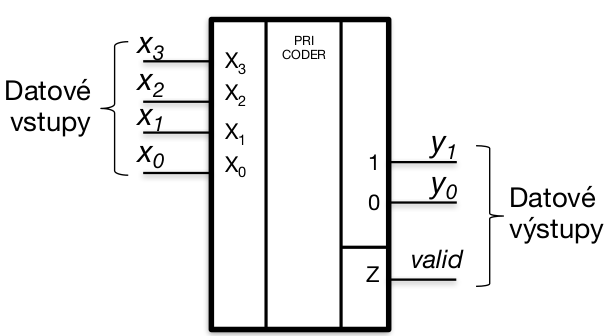
\includegraphics[width=\textwidth]{img/PrioEn.png}
    \end{minipage}
    \hfill
    \begin{minipage}[b]{0.4\textwidth}
        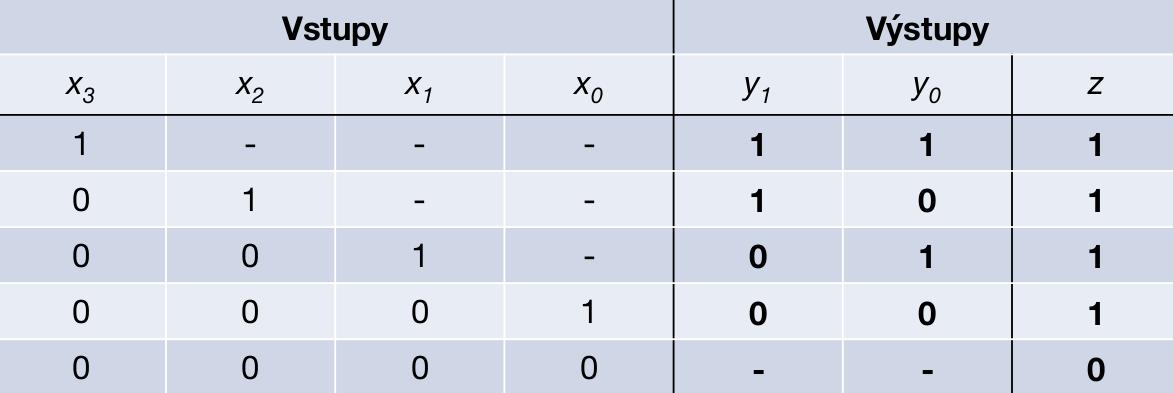
\includegraphics[width = \textwidth]{img/PriEnTab.png}
    \end{minipage}
\end{figure}

\subsection{Číslicový komparátor}
Porovnává 2 čísla v binárním kódu. \\
Nejčastěji dává informaci o shodě dvou čísel - porovnání dvojce bitů na stejné pozici.\\
Existují i komparátory, vyhodnocující na dalších dvou výstupech výsledky operaci (A > B) a (A < B).\\
\begin{figure}[h!]
    \centering
    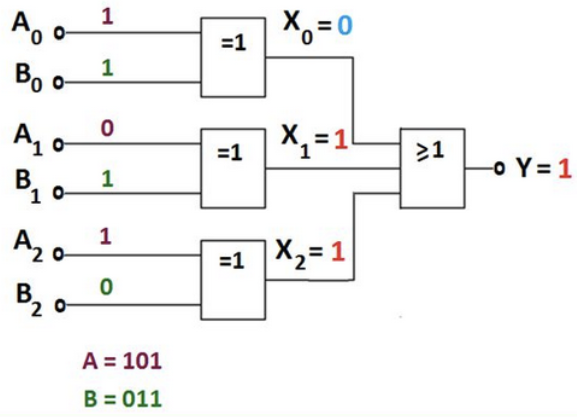
\includegraphics[scale = 0.3]{img/Kompar.png}
\end{figure}

\subsection{Binární sčítačka}
Sčítá dvě čísla v binárním kódu - výsledek je číslo v binárním kódu a přenos do vyššího řádu.\\
Pro vícebitové čísla kaskáda jednobitových sčítaček.\\
Odčítačky jsou realizovány podobně, akorát je jedna ze vstupních hodnot binárně invertována a na vstupu \(c_0\) je hodnota nastavena jako logická 1. \\
\subsubsection{Poloviční sčítačka - Half Adder}
\begin{figure}[h!]
    \centering
    \begin{minipage}[b]{0.4\textwidth}
        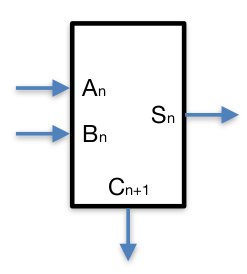
\includegraphics[scale = 0.5]{img/HA.png}
    \end{minipage}
    \hfill
    \begin{minipage}[b]{0.4\textwidth}
        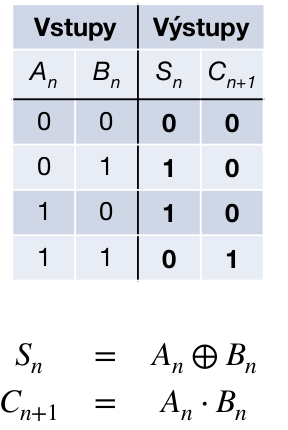
\includegraphics[scale = 0.3]{img/HATab.png}
    \end{minipage}
\end{figure}
\subsubsection{Plná sčítačka - Full Adder}
\begin{figure}[h!]
    \centering
    \begin{minipage}[b]{0.4\textwidth}
        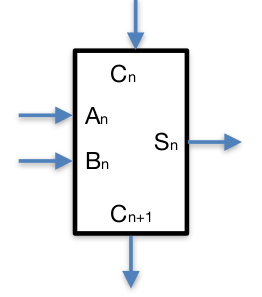
\includegraphics[scale = 0.5]{img/FA.png}
    \end{minipage}
    \hfill
    \begin{minipage}[b]{0.4\textwidth}
        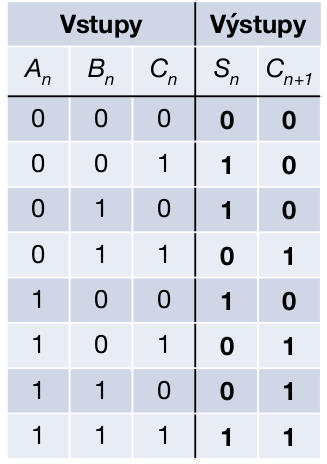
\includegraphics[scale = 0.3]{img/FATab.png}
    \end{minipage}
\end{figure}

\begin{figure}[h!]
    \centering
    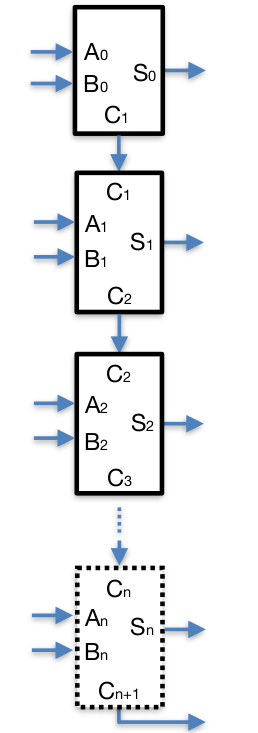
\includegraphics[scale=0.3]{img/Ripple-carry.png}
\end{figure}

\subsubsection{Binární odčítačka}
Podobná sčítačce, ale používáme druhý doplněk. Pokud A<B pak je výsledek ve druhém doplňku, pokud je A>B, je výsledek kladný.\\
\(A-B = A + \lnot B + 1\).\\

\subsection{Druhý doplněk}
Způsob kódování celých čísel do binárního kódu. \\
Převod do něj se provádí přes převod čísla do 1. doplňku, což je to stejné jako inverze bitů a následně k invertovanému číslu přičteme 1.
\begin{center}
    1. binární kód: 0101 1001\\
    2. 1. doplněk:  1010 0110\\
    3. 2. doplněk:  1010 0111\\
\end{center}
Odčítání pomocí 2. doplňku se provádí následovně:
\begin{center}
    Mějme 2 čísla: 1000 0001 a 11 0110.\\
    1. Zarovnáme počet bitů: 11 0110 -> 0011 0110\\
    2. provedeme inverzi menšitele: 0011 0110 -> 1100 1001\\
    3. Zvýšíme menšitele o 1: 1100 1001 -> 1100 1010\\
    Následně již provedeme součet.
\end{center}
\subsection{Logické obvody s třístavovým výstupem}
Fungují ve dvojkové soustavě (0 a 1), kterým se přiřazují pevné napěťové úrovně L a H.\\
Třetí stav, kterého může logický člen nabýt je stav vysoké impedance. Člen odpojí svůj výstupní port a neovládá ho. Výstup tedy není konkrétně definován a může nabývat libovolného stavu, který může být řízen jiným členem.\\
Využívány pokud je výstup obvodů připojen na společnou sběrnici s jinými výstupy. Musíme řídit, který signál po sběrnici jde.\\
Tato volba se dělá ovládacím signálem chip select (CS), který výstup povoluje, pokud není povolen tak je obvod ve stavu vysoké impedance.\\

\subsection{Logické obvody s otevřeným kolektorem}
Výstup tvořen pouze jedním NPN tranzistorem(normálně tvořen párem tranzistorů), který spíná výstup ke společnému potenciálu. \\
Báze je připojena k internímu logickému členu, takže stav členu i výstupního tranzistoru závisí na vstupních signálech a funkci konkrétního integrovaného obvodu. \\
Tranzistor buď není sepnut a kolektor není spojen s žádným potenciálem, nebo je sepnut a kolektor je spojen se zemí. Kotevřenému kolektoru se obvykle připojuje pull up rezistor(1-10kΩ), který zajišťuje logickou úroveň H v případě, že tranzistor není sepnut, v případě L je tranzistor sepnut a výstup spojen se zemí.

\begin{figure}[h!]
    \centering
    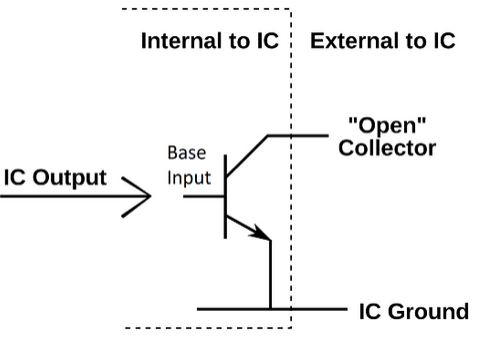
\includegraphics[scale = 0.5]{img/OpenColl.png}
\end{figure}

\subsection{Připojování zařízení na sběrnici}
Se zařízením na sběrnici komunikuje řadič instruovaný procesorem. Na jedné sběrnici může být více zařízení.\\
Šířka sběrnice je počet drátů sběrnice.\\
Rychlost je počet bitů přenesených za 1 sekundu na jednom drátě.\\
Šířka pásma je objem dat za jednotku času.\\
Nesdílená sběrnice, má zvlášť dráty pro data, adresy, řízení. Společná má vodiče sdílené pro adresy a data.\\

\section{Přechodné děje v kombinačních logických obvodech, hazardní stavy (souběhový, dynamický a statický hazard), metody detekce a řešení statického hazardu ve dvoustupňové struktuře NAND-NAND, konsensus, řešení hazardu pomocí sekvenčních obvodů.}

\subsection{Přechodné děje v kombinačních logických obvodech}
\subsubsection{Zpoždění změny výstupu}
Při změně vstupního stavu má na výstupu dojít ke změně (0 a 1).\\
Vyšetřujeme krajní hodnoty zpoždění změny signálu na výstupu.\\
Symbolika:
\begin{itemize}
    \item Hodnota vstupu nemá vliv na výstup: \(\widetilde{a}\)
    \item Změna vstupu z 0 do 1: \(a_{\uparrow}\)
    \item Změna vstupu z 1 do 0: \(a_{\downarrow}\)
    \item Střídavá změna: \(a_{\updownarrow}\)
\end{itemize}
Nelze předpokládat stejnou dobu přechodu z 0 do 1 a z 1 do 0. Obecně \(t_{pLH} > t_{pHL}\).\\
Zpoždění ovlivňuje hodnota zpoždění hradla, ale také délka cesty signálu. \\
\begin{figure}[h!]
    \centering
    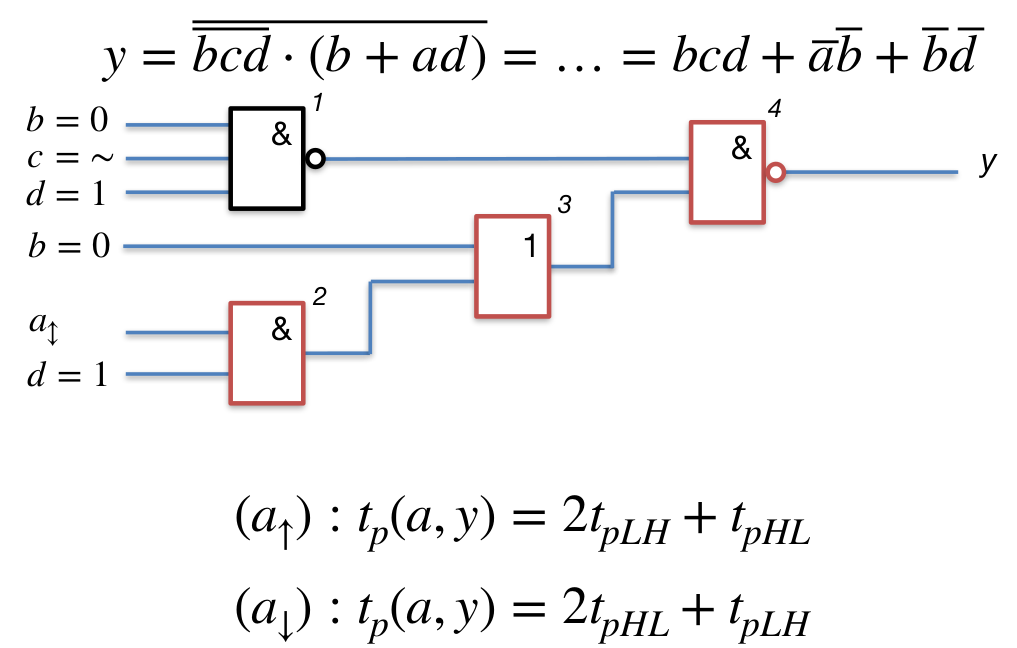
\includegraphics[scale = 0.3]{img/PrechDej.png}
\end{figure}

\subsubsection{Vznik glitche a hazard}
Při změně vstupního stavu má být na výstupu neměnná hodnota.\\
Pří některý změnách vstupních stavů, ale dochází na výstupu ke vzniku, krátkých falešných impulzů (glitche). Vstupní stavy, při kterých se tyto falešné impulzy projeví, se nazývají hazardní stavy (hazardy).\\
Při přechodných dějích neplatí pravidla booleovy algebry o kompelemtech \(a + \overline{a} = 1, a\cdot \overline{a} = 0\). Neplatí pravidla spojování termů \(ab + a\overline{b} = a(b + \overline{b})\). Ani pravdila absorpce \(a + (\overline{a} \cdot b)= (a + \overline{a})\cdot (a + b)\).\\

\subsection{Rozdělení hazardů}
\subsubsection{Souběhový hazard}
Nastává při změně více vstupních proměnných ve stejný okamžik, proto je snaha o změnu jedné vstupní proměnné naráz.
\newpage
\begin{figure}[h!]
    \centering
    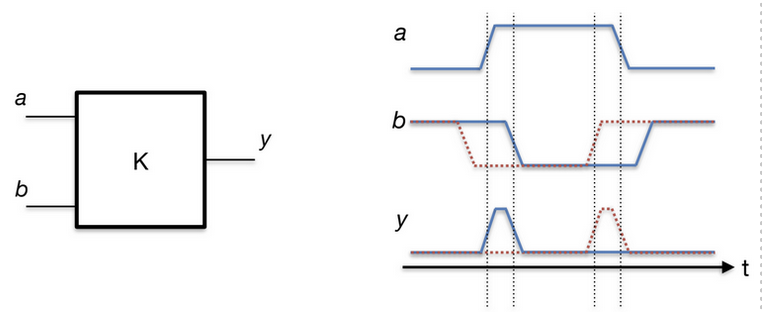
\includegraphics[scale = 0.5]{img/SoubehH.png}
\end{figure}

\subsubsection{Statický hazard}
Předpokládáme konstantní výstup, ale vznikne glitch.\\
\begin{figure}[h!]
    \centering
    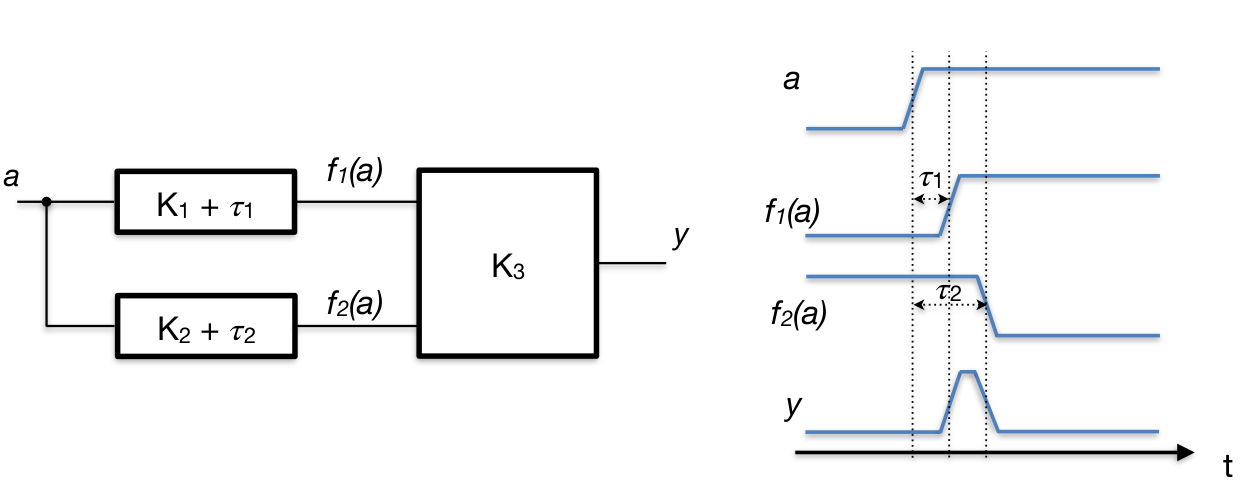
\includegraphics[scale= 0.3]{img/StatH.png}
\end{figure}

\subsubsection{Dynamický hazard}
Předpokládáme jednu změnu výstupu, ale dojde k vygenerování více změn výstupu(vždy ale o lichém počtu).\\
\begin{figure}[h!]
    \centering
    \includegraphics*[scale = 0.3]{img/DynH.png}
\end{figure}

\subsubsection{Předpoklady pro eliminaci statického hazardu}
Předpokládáme změnu pouze jedné vstupní proměnné.\\
Předpokládáme dvoustupňovou strukturu kombinační logické funkce, NAND-NAND nebo NOR-NOR.\\
Za těchto předpokladů můžeme hazard eliminovat.\\
\subsection{Metody detekce a řešení statického hazardu ve dvoustupňové struktuře NAND-NAND}
Hazard lze eliminovat úpravou kombinačního obvodu.\\
\subsubsection{Pomocí Karnaughovy mapy}
\begin{figure}[h!]
    \centering
    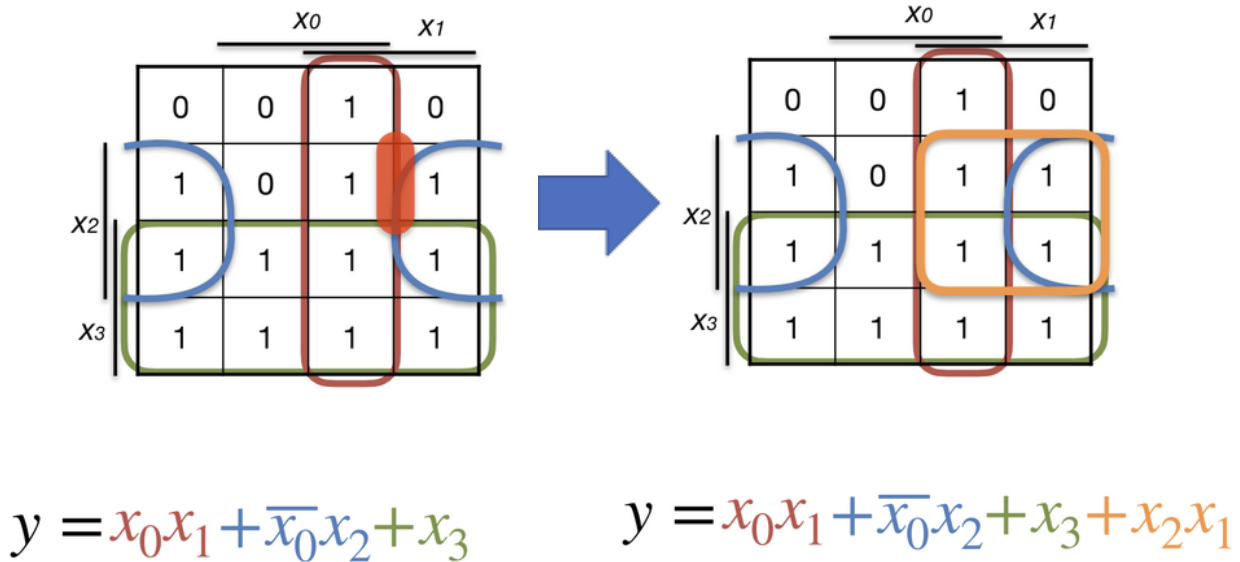
\includegraphics[scale = 0.2]{img/ElimHazKM.png}
\end{figure}

\subsubsection{Pomocí booleovy algebry}
Předpokládejme kombinační logický obvod: \(y = f(x_n,x_{n-1},...,x_0)\).\\
Vyšetřujeme přítomnost hazardu při změně proměnné \(x_0\).\\
Upravme výraz na: \(y = x_0\cdot A + \overline{x_0}\cdot B + C\)
Hazard pak exituje pouze pokud platí že pro zbývající hodnoty vstupních proměnných je možná dosáhnout následujících podmínek: A=1, B=1, C=0, tedy \(A\cdot B \cdot \overline{C} = 1\).\\
Pokud v původní funkci hazard je, musíme aplikovat boolovské pravidlo konsenzus: \(y = x_0 + \overline{x_0}B + C + A\cdot B\)\\
Výraz pak již není minimální, ale neobsahuje hazard.\\

\subsubsection{Další metody potlačení glitche}
Pomocí filtru(naivní řešení), pouze jako nouzové řešení, vhodné jako dočasná oprava chyb při návrhu kombinačního filtru.\\
Potlačení glitche pomocí registru(využití sekvenčních obvodů), na obrázku.\\
\begin{figure}[h!]
    \centering
    \includegraphics*[scale = 0.5]{img/HazElim.png}
\end{figure}
Pomocí zpožďovacího členu v obvodu, nepoužívá se.

\section{Rozdíl mezi kombinačním a sekvenčním logickým obvodem. Klopné obvody: RS, D, JK, T, hladinové, hranové a master-slave, pravdivostní tabulka, pojem metastabilita v sekvenčních logických obvodech.}
\subsection{Rozdíl mezi kombinačním a sekvenčním logickým obvodem}
\subsubsection{Kombinační obvody}
Kombinace hodnot výstupních signálů v daném okamžiku je dána pouze kombinací hodnot vstupních signálů v tomto okamžiku. Aktuální výstupní kombinace nezávisí na vstupních kombinacích v minulosti.\\
Typické obvody: hradla, multiplexory, demultiplexory, dekodéry, enkodéry, atd.

\subsubsection{Sekvenční obvody}
Kombinace hodnot výstupních signálů v daném okamžiku je určena jednak kombinací hodnot vstupních signálů v tomto okamžiku, ale i kombinacemi vstupních signálů v předcházejících okamžicích.\\
Sekvenční obvod má vnitřní paměť.\\

\subsection{Klopné obvody}
Obvody, které se mohou nacházet ve dvou stabilních rovnovážných stavech, v nichž se obvodové veličiny(napětí a proud) v obvodu nemění.\\
Tyto stavy můžou být stabilní trvale, přechod do druhého stavu nastane pouze při vnějším podnětu, nebo jsou stabilní dočasně - ke změně dojde stavu dojde spontánně po uplynutí definované doby.\\
Podle charakteru stabilních rovnovážných stavů se klopné obvody dělí na:
\begin{itemize}
    \item Bistabilní(BKO) - oba stavy trvale stabilní
    \item Monostabilní(MKO) - jeden stav je stabilní trvale a jeden dočasně
    \item Astabilní(AKO) - oba jsou dočasně stabilní
\end{itemize}
BKO neměřeí čas, MKO a AKO vytváří impuly, odměřují čas.\\
Kromě dvou stabilních rovnovážných stavů(A,B) existuje v klopných obvodech ještě nestabilní rovnovážný stav (C), z něhož obvod při sebemenší výchylce přejde do některého ze stabilních rovnovážných stavů.\\
\subsubsection{Konstrukce sekvenčních obvodů}
Sekvenční obvody obsahují jistý druh paměti, ta je realizována buď setrvačnými prvky(L,C) v AKO a MKO, které odměřují čas. V BKO je paměť realizována kladnými zpětnými vazbami, neodměřuje čas, při známé časové periodě impulzů, lze tento nedostatek obejít.\\

\subsection{Synchronní a asynchronní sekvenční obvody}
\subsubsection{Synchronní}
Mohou měnit svůj stav jen v časových okamžicích, které jsou určeny speciálním hodinovým signálem.\\
Tyto obvody obsahují hodinové vstupy - ty jsou u synchronních systémů všechny paralelně propojeny.\\
\subsubsection{Asynchronní}
Mění svůj stav v libovolném časovém okamžiku.\\
Nemají hodinové vstupy, případně je nemají paralelně propojeny.\\

\subsection{Asynchronní klopné obvody}
\subsubsection{Asynchronní RS}
Bistabilní klopný obvod se vstupem Set pro nastavení výstupu Q na hodnotu 1 a vstupem Reset pro nastavení výstupu Q na hodnotu 0. Při kombinaci na vstupech (R = S = 0), se obvod chová jako Bus Hold – realizuje paměť.\\

\begin{figure}[h!]
    \centering
    \begin{minipage}[b]{0.4\textwidth}
        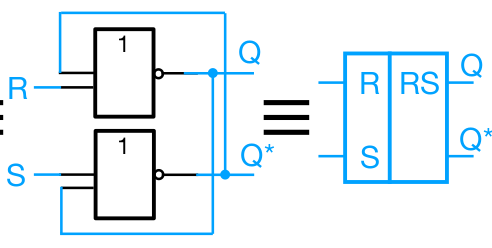
\includegraphics[scale = 0.4]{img/RSor.png}
    \end{minipage}
    \hfill
    \begin{minipage}[b]{0.4\textwidth}
        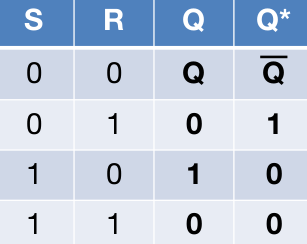
\includegraphics[scale = 0.3]{img/RSTab.png}
    \end{minipage}
\end{figure}

Kombinace vstupů (R = S = 1) je problematická ze dvou důvodů. Kromě této kombinace jsou výstupy Q a Q* vždy komplementární. Nelze zjistit hodnoty výstupů Q a Q* při přechodu z (R = S = 1) do (R = S = 0) tzv. Metastabilní stav/děj.\\

\begin{figure}[h!]
    \centering
    \includegraphics*[scale = 0.4]{img/RSMeta.png}
\end{figure}
Výstupní signály jsou jednoznačně určeny až do okamžiku, kdy se oba signály R a S současně mění z 1 -> 0. Pokud je obvod dokonale souměrný, mají oba výstupy snahu přecházet do 1. Po přechodu obou těchto signálů přes prahovou úroveň mají ale opětovně oba signály snahu vrátit se zpět do 0. Tímto způsobem může vzniknout kmitání v oblasti prahové úrovně. Nakonec drobné nesymetrie v reálných obvodech převáží a způsobí výsledný rozdíl v obou výstupních signálech - nelze odhadnout výsledné hodnoty ani dobu metastabilního děje! (děj bývá obecně delší, než běžná změna stavu).

Realizace pomocí NAND. Pro zachování tabulky je nutné negovat vstupní signály R a S, vyměnit označení R a S. Při (R = S = 1) je nyní výstup (Q = Q* = 1), při přechodu z (R = S = 1) do (R = S = 0) opět metastabilní stav.

\begin{figure}[h!]
    \centering
    \includegraphics*[scale = 0.5]{img/RSNAND.png}
\end{figure}

\subsection{Hladinové synchronní klopné obvody}
\subsubsection{Synchronní RS pomocí NAND}
Pro signál C=0 realizuje paměť a pro C=1 se chová jako asynchronní RS.\\
\begin{figure}[h!]
    \centering
    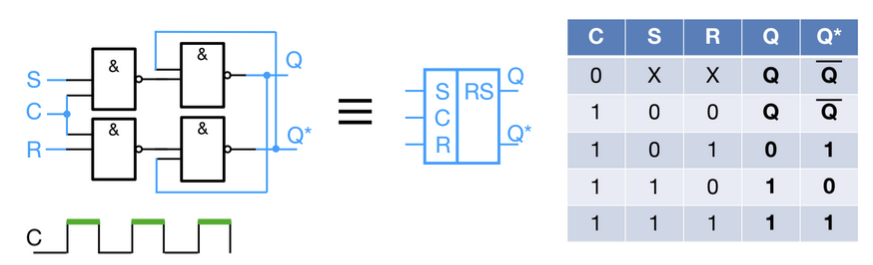
\includegraphics[scale = 0.5]{img/HladRS.png}
\end{figure}

\subsubsection{Hladinový synchronní klopný obvod D pomocí RS}
Transparent latch, při C = 1 promítá vstup D na výstup Q, pro C = 0 realizuje paměť.\\
Vyřešen problém s metastabilitou.\\
\newpage
Zápis v booleově algebře
\begin{center}
    \(Q^t = D^{t-1} = C\cdot D + \overline{C} \cdot Q^{t-1} + D \cdot Q^{t-1}\)
\end{center}

\begin{figure}[h!]
    \centering
    \includegraphics*[width = \textwidth]{img/Dlatch.png}
\end{figure}

\subsubsection{Hladinový synchronní klopný obvod D ve zpětné vazbě}
Vzaba výstupu \(\overline{Q}\) na vstup D.\\
C = 0 paměť, C = 1 na výstupu neznámá hodnota.\\
\begin{figure}[h!]
    \centering
    \includegraphics*[scale = 0.5]{img/Dzv.png}
\end{figure}

\subsection{Hranové synchronní klopné obvody}
\subsubsection{Hranový synchronní klopný obvod RS: Master-Slave}
Označení Synchronního RS, který reaguje na nástupnou či sestupnou hranu.\\
\begin{figure}[h!]
    \centering
    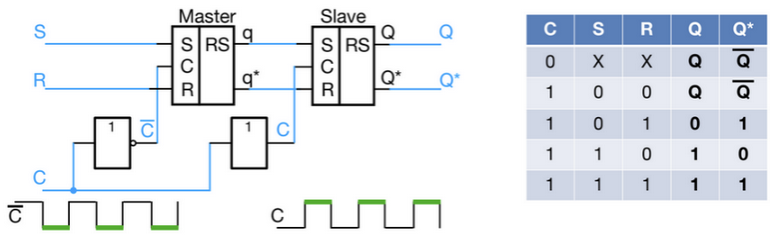
\includegraphics[scale = 0.5]{img/MS.png}
\end{figure}
\newpage
Značení Master-slave s nástupnou/sestupnou hranou:
\begin{figure}[h!]
    \centering
    \begin{minipage}[b]{0.4\textwidth}
        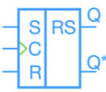
\includegraphics[width = \textwidth]{img/MSup.png}
    \end{minipage}
    \hfill
    \begin{minipage}[b]{0.4\textwidth}
        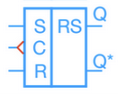
\includegraphics[width = \textwidth]{img/MSdown.png}
    \end{minipage}
\end{figure}

\subsubsection{Hranový sychnronní klopný obvod D}
Registr. \\
Po nástupné hraně bude na Q hodnota D z doby před náběžnou hranou. \\
Jindy se chová jako paměť.\\
\begin{figure}[h!]
    \centering
    \includegraphics*[scale = 0.5]{img/DHran.png}
\end{figure}

\subsubsection{Hranový synchronní klopný obvod JK}
Vhodný pro tvorbu čítačů.\\
Pomocí J a K lze vytvořit: Paměť, reset, set, negace paměti.\\
\begin{figure}[h!]
    \centering
    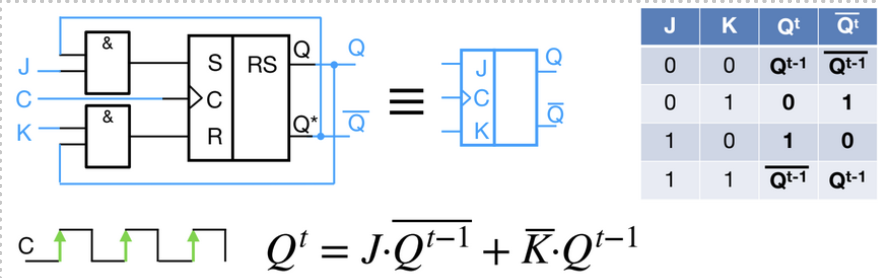
\includegraphics[scale = 0.5]{img/JK.png}
\end{figure}

\subsubsection{Hranový synchronní klopný obvod T}
Zjednodušený JK, vhodný pro čítače. Reálně vždy potřebuje více vstupů, alespoň asynchronní reset. \\
\begin{figure}[h!]
    \centering
    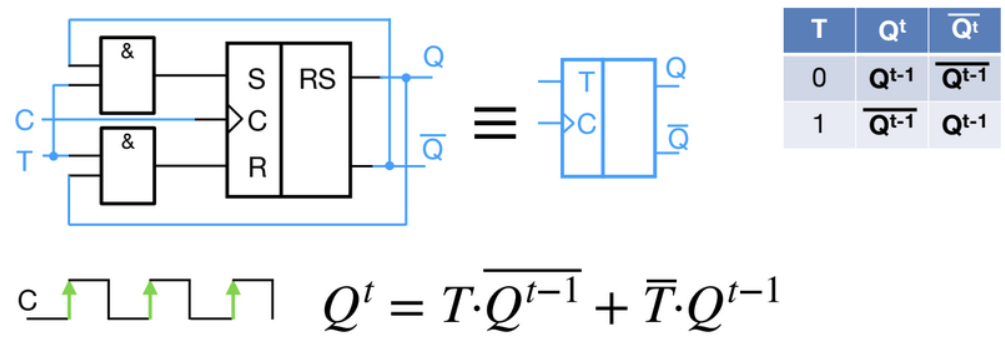
\includegraphics[scale = 0.3]{img/T.png}
\end{figure}

\section{Sekvenční logické obvody: posuvný registr, posuvné registry se zpětnou vazbou (kruhový čítač, Johnsonův čítač, lineární čítač - LFSR), asynchronní a synchronní čítače, popis jejich funkce pomocí jazyka HDL. Vysvětlete pojmy HDL jazyka: souběžný a sekvenční příkaz, okamžité a odložené přiřazení.}
\subsection{Sekvenční logické obvody}
\subsubsection{Posuvný registr}
Skupina obvodů sestavená tak, že s náběžnou hranou se bity posunou o jeden klopný obvod.\\
\begin{figure}[h!]
    \centering
    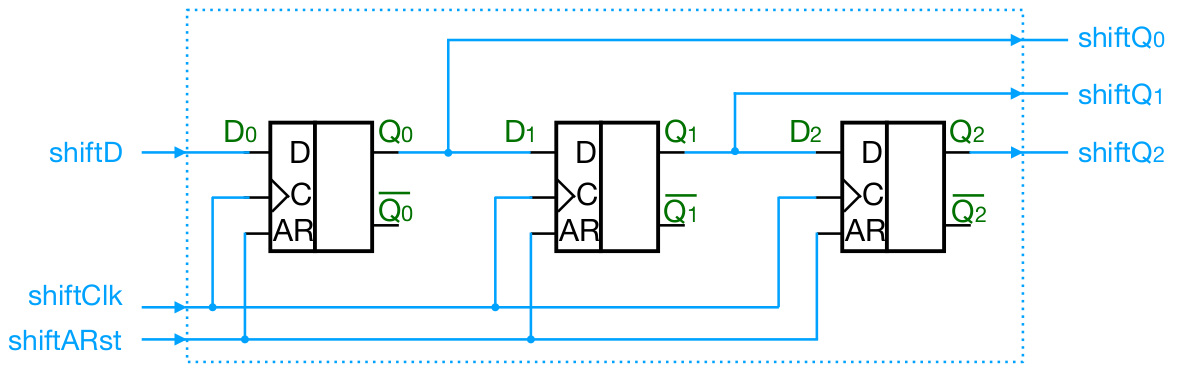
\includegraphics[scale = 0.3]{img/PosuvReg.png}
\end{figure}
\begin{figure}[h!]
    \centering
    \includegraphics*[scale = 0.3]{img/CasPosuv.png}
\end{figure}
\newpage
Impuls CLK je shodný pro všechny klopné obvody (KO) posuvného registru. Po jeho náběžné hraně se (se zpožděním \(t_{Ddelay}\) ) překlopí první KO D0, ale pro druhý KO D1 musí být signál \(D_1\) stabilní ještě po dobu přesahu \(t_{hold}\). Dále musí být signál \(D_1\) stabilní alespoň po dobu \(t_{setup}\) před další náběžnou hranou signálu CLK. Proto tedy musí platit:
\begin{center}
    \(t_{Ddelay} \geqq t_{hold}\)\\
    \(T_{clk} \geqq t_{Ddelay} + t_{setup}\)
\end{center}

Obecné schéma posuvného registru:\\
\begin{figure}[h!]
    \centering
    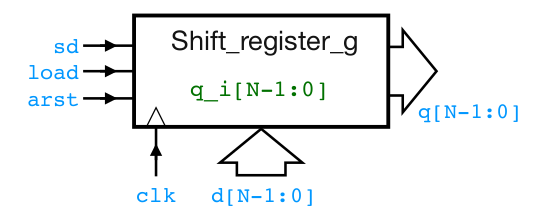
\includegraphics[scale = 0.5]{img/ShiftReg.png}
\end{figure}

Implementace jednosměrného posuvného registru:\\
\begin{lstlisting}
    ENTITY Shift_register_g IS
        GENERIC(N: positive := 4);
        PORT(
            clk, sd, load, arst: IN std_logic;
            d:                   IN std_logic_vector(N-1 DOWNTO 0);
            q:                   OUT std_logic_vector(N-1 DOWNTO 0)
            );
    END Shift_register_g;
    ARCHITECTURE Behavioral OF Shift_register_g IS
        SIGNAL q_i: std_logic_vector(N-1 DOWNTO 0)
    BEGIN
        PROCESS(arst, clk)
        BEGIN
            IF(arst = '1') THEN
                q_i <= (OTHERS => '0');            --Async reset
            ELSIF rising_edge(clk) THEN
                IF(load = '1') THEN                --Sync parallel load
                    q_i <= d;
                ELSE
                    q_i <= q_i(N-2 DOWNTO 0) & sd; --Sync serial shift
                END IF;
            END IF;
        END PROCESS;
        q <= q_i;
    END ARCHITECTURE Behavioral;
\end{lstlisting}

Implementace obousměrného posuvného registru:\\
\begin{lstlisting}
    ENTITY Shift_reg_bidir_g IS
        GENERIC(N: positive := 8);
        PORT(
            sd, dir, arst, clk:  IN std_logic;
            q:                   OUT std_logic_vector(N-1 DOWNTO 0)
            );
    END Shift_reg_bidir_g;
    ARCHITECTURE Behavioral OF Shift_reg_bidir_g IS
        SIGNAL q_i: std_logic_vector(N-1 DOWNTO 0)
    BEGIN
        PROCESS(arst, clk)
        BEGIN
            IF(arst = '1') THEN
                q_i <= (OTHERS => '0');            --Async reset
            ELSIF rising_edge(clk) THEN
                IF(dir = '1') THEN
                    q_i <= q_i(N-2 DOWNTO 0) & sd; --Sync serial shift left
                ELSE
                    q_i <= sd & q_i(N-1 DOWNTO 1); --Sync serial shift right
                END IF;
            END IF;
        END PROCESS;
        q <= q_i;
    END ARCHITECTURE Behavioral;
\end{lstlisting}

\subsubsection{Kruhový registr}
Data, předem vložená do posuvného registru, potom neustále rotují o jeden bit s každým hodinovým impulzem.\\
Data lze do registru vkládat sériově nebo paralelně (paralelní vstupy). Nemusí obsahovat obě varianty.\\
Volbou vhodné počáteční hodnoty lez dosáhnout až periodů danou počtem bitů registru N.\\
\begin{figure}[h!]
    \centering
    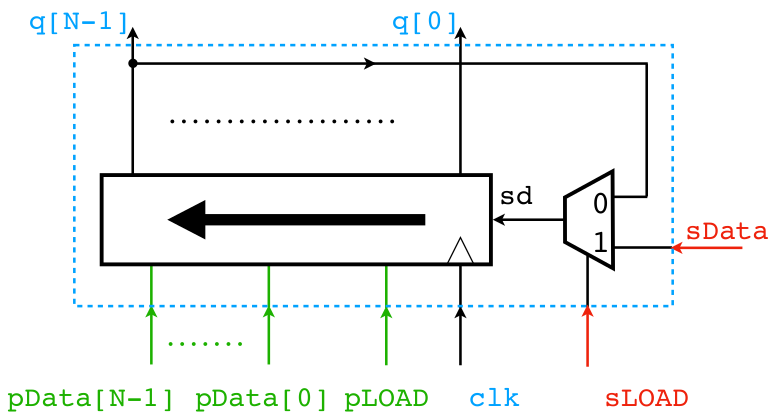
\includegraphics[scale = 0.4]{img/KruhCt.png}
\end{figure}

\subsubsection{Johnsonův čítač}
Volbou vhodné inicializační hodnoty obsahující ve všech bitech stejné hodnoty, lze zajistit periodu danou dvojnásobným počtem bitů posuvného registru.
\begin{figure}[h!]
    \centering
    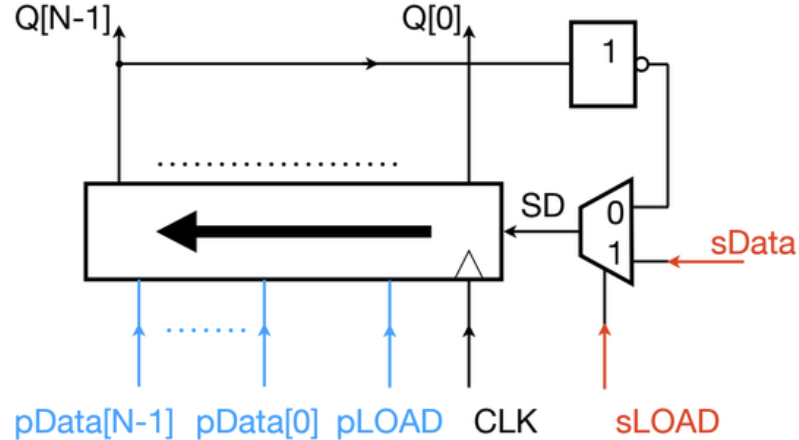
\includegraphics[scale = 0.4]{img/Johnson.png}
\end{figure}

\subsubsection{Lineární čítač}
Linear-feedback shift register - LFSR.\\
Složitější kombinační obvod ve zpětné vazbě XOR.\\
Platí pravidlo „pro libovolnou délku lze nalézt aspoň jednu kombinaci odboček do funkce XOR tak, že posloupnost výstupů je dlouhá 2N-1“ což je posloupnost maximální délky.\\
Jediná hodnota které není dosažitelná jsou samé 0, při tomto výstupu totiž obvod již navždy zůstane v tomto stavu. Proto nutno nastavit na nenulovou hodnotu.\\
Funguje jako generátor liché parity.\\
\begin{figure}[h!]
    \centering
    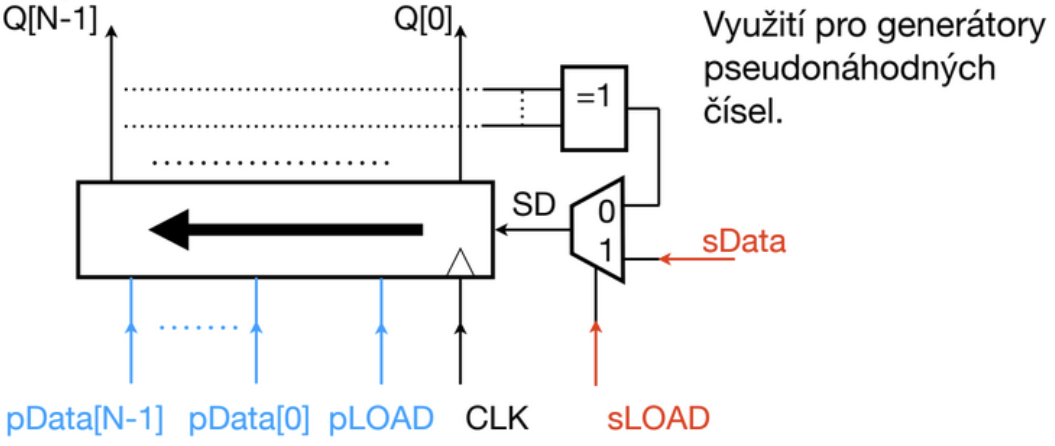
\includegraphics[scale = 0.4]{img/LSFR.png}
\end{figure}
\newpage
Odbočky jednotlivých bitů se vyjadřují polynomem: \(x^{N-1}+...+x^1+x^0\). Volbou těchto odboček určujeme sekvenci výstopních hodnot a jejich periodu.\\
Použití v kryptografii jako proudová šifra. \\
2 základní konstrukce - Fibonacci a Galois.\\
Fibonacci LFSR: \\
\begin{figure}[h!]
    \centering
    \includegraphics*[scale = 0.4]{img/Fibonacii.png}
\end{figure}

Galois LFSR: \\
\begin{figure}[h!]
    \centering
    \includegraphics*[scale = 0.4]{img/Galois.png}
\end{figure}

Fibonacci i Galois mohou generovat stejné sekvence a jsou zaměnitelné, ale musí být incializovány jinými hodnotami.\\
Jedničky a nuly se střídají v tvz. bězích. Například 1110010 má 4 běhy o délkách 3,2,1,1. Vždy jedna polovina běhů má délku 1, čtvrtina délku 2, a tak dále až k jednomu běhu délky N.
Výstupní proud je deterministický, pokud známe aktuální vnitřní hodnoty, délku registru a místa odbořek jsme schopni predikovat další výstup.\\
Používají se jako generátory pseudonáhodných čísel.

\subsection{Synchronní a asynchronní čítač}
Slouží k počítání impulsů. Čítač po každém impulsu mění stav a postupně prochází cyklem M stav. Poté se cyklus opakuje, celkový počet opakování nejde zjistit.\\
Využití: detekce počtu impulsů, deličky kmitočtu.\\

\begin{figure}[h!]
    \centering
    \includegraphics*[scale = 0.3]{img/citace.png}
\end{figure}
Dělení čítačů:
\begin{itemize}
    \item Dle distribuce hodinového signálu
          \begin{itemize}
              \item Asynchronní
              \item Synchronní
          \end{itemize}
    \item Dle směru
          \begin{itemize}
              \item Dopředné
              \item Zpětné
              \item Vratné(reverzibilní)
          \end{itemize}
    \item Dle směru používaného kódu
          \begin{itemize}
              \item Binární
              \item BCD - Binary coded decimal
              \item Modulo M
              \item Grayově kódu
          \end{itemize}
\end{itemize}
\subsubsection{Asynchronní čítače}
Clk přiveden jen na první klopný obvod.\\
Překlápění probíhá postupně od LSB k MSB.\\
Dnes méně využívány, vhodné pro aplikace
nenáročné na vzájemně přesné časové průběhy.\\
Velké zpoždění.\\
Menší počet komponent, žádné propojovací obvody.\\
Pouze první klopný obvod musí být schopen pracovat na frekvenci hodinového signálu.\\
\begin{figure}[h!]
    \centering
    \includegraphics*[scale = 0.5]{img/AsynCit.png}
\end{figure}

\subsubsection{Synchronní čítače}
Clk přiveden na všechny klopné obvody.\\
Všechny klopné obvody musí být schopné pracovat na frekvenci hodinového signálu. Překlápění probíhá na všech paralelně.\\
Větší počet komponent, nejen propojené klopné obvody, ale i kombinační část realizující paralelní výpočet nového stavu.\\
Oddělená paměťová(registrová) a kombinační část - výhodné i pro stavové automaty.\\
Umístěny v kaskádě. Využívá se vstup CE, clock enable, který povoluje čítání. Celá kaskáda obsahuje signály CE a CEO, clock enable output, který povoluje čítání další kaskády. Bývá zde ještě signá TC, terminal Count, který podává informaci, že čítač dosáhl své maximální hodnoty a při příští změně začne od začátku.\\
\begin{figure}[h!]
    \centering
    \includegraphics*[scale = 0.4]{img/SyncCit.png}
\end{figure}

Blok synchronního čítače je následující: \\
\begin{figure}[h!]
    \centering
    \includegraphics*[scale = 0.5]{img/Sync.png}
\end{figure}

Implementace synchronního čítače:\\
\begin{lstlisting}
    LIBRARY ieee;
    USE ieee.std_logic_1164.ALL;
    USE ieee.numeric_std.ALL;            -- pro konverzi na std_logic_vector
    ENTITY Counter_binary IS
        PORT(
            clk: IN std_logic;
            q : OUT std_logic_vector(2 DOWNTO 0)
        );
    END Counter_binary;
    ARCHITECTURE Behavioral OF Counter_binary IS
        SIGNAL d_i, q_i: unsigned(q'range) := (OTHERS => '0');
    BEGIN
        PROCESS(clk)
        BEGIN
            IF rising_edge(clk) THEN
                q_i <= d_i;             
            END IF;
        END PROCESS;
        PROCESS(q_i)
        BEGIN
            d_i <= q_i + 1;
        END PROCESS;
        q <= std_logic_vector(q_i); -- unsigned na std_logic_vector
    END ARCHITECTURE Behavioral;
\end{lstlisting}

\subsubsection{VHDL implementace čítače}
Výsledná realizace obsahuje na ýstupech TC a CEO kombinační obvody, které mohou generovat hazardy.\\
Je důležité zhodnotit, zda daná situace je nebo není na závadu. Hazardy není potřeba řešit = následující blok je synchronní s CLK. Hazardy je nutné řešit = následující blok není synchronní. Na výstupy přidáme záchytné registry, které zajistí jejich změny s CLK, ale zpozdí je o jednu periodu hodinového signálu CLK.\\

\subsection{Souběžný a sekvenční příkaz}
\subsubsection{Souběžný}
Příkazy probíhají zároveň a nezáleží na jejich pořadí ve zdrojovém textu.\\
\subsubsection{Sekvenční}
Příkazy probíhají postupně a záleží na jejich pořadí ve zdrojovém textu.\\
\subsection{Okamžité a odložené přiřazení}
\subsubsection{Okamžité :=}
Platí pouze uvnitř procesu pouze pro proměnné.\\
\subsubsection{Odložené <= }
Platí pro signály.\\
Pokud jsou v těle procesu postupně přiřazovány jednomu signálu různé hodnoty, má signál hodnotu odpovídající poslednímu přiřazovacímu příkazu. Přičemž až do konce procesu má signál vždy svoji původní hodnotu.\\
Lze si to představit tak, že k přiřazení všech hodnot signálům dojde najednou až v okamžiku skončení procesu.\\

\section{Konečné stavové automaty: Obecný (Huffmanův) model sekvenčního logického obvodu, přechodová funkce, výstupní funkce, budicí funkce. Mealyho, Mooreho a autonomní automat. Popis konečného automatu pomocí stavového diagramu, tabulky přechodů a tabulky výstupů. Návrhová tabulka (budicí funkce KO).}

Nejobecnější model každého sekvenčního obvodu je konečný stavový automat(KSA). Tento obvod má konečný počet vstupních stavů, výstupních stavů i vnitřních stavů. \\
Stav je kombinace hodnot signálů - v technické praxi pracujeme s binárními signály.\\
Každou kombinaci kvůli úspornosti označujem písmenem/symbolem.\\
KSA popisuje velice jednoduchý počítač, který může být v jednom z několika vnitřních stavů.\\
Mezi stavy přechází na základě symbolů čtených ze vstupu.\\
KSA si pamatuje pouze vnitřní stav.\\
Symbol je nedělitelná jednotka, se kterou pracujeme - písmeno, číslice, 0 a 1.\\
Abeceda je libovolná konečná neprázdná množina symbolů. Značí se \(\Sigma \). Příklady: binární abeceda \(\Sigma = \{0,1\} \), \(\Sigma = \{+,-,0,1,2,3,4,5,6,7,8,9\} \).\\
Slovo je libovolná konečná posloupnost symbolů dané abecedy.\\
Formální jazyk libovolná množina slov vytvořených nad abecedou \(\Sigma \), značíme jej písmenem L, konečný jazyk má končený počet slov, nekonečný nemá. Abeceda = (a, b, c) => jazyk L1 = (a, bb, ac, bc), jazyk L2 = (abc, bca, cba).\\

\subsection{Rozpoznávací KSA}
KSA bez výstupu, výstupem je jeho vnitřní stav. Umožňuje příjmout nebo zamítnout dané slovo. \\
\(A = (Q, \Sigma, \delta, q_0, F) \), kde Q je množina vnitřních stavů, \(\Sigma \) je množina vstupních symbolů, \(\delta \) je stavově přechodová funkce, \(q_0\) je počáteční vnitřní stav, F je množina koncových stavů.
Použití: rozpoznávání řetězců z L, detekce chyb.\\

\subsection{Synchronní a asynchronní automaty}
Mezi současným a následujícím vnitřním stavem musí existovat časový odstup.\\
\subsubsection{Asynchronní automaty}
Časový odstup mezi stavy je pouze důsledkem zpoždění vnitřních obvodů vytvářejících stavové signály.\\
Mění svůj vnitřní stav (s malým zpožděním) po změně vstupního stavu.\\
\subsubsection{Synchronní automaty}
Okamžik změny vnitřního stavu je určen synchronizačními impulsy(hodinovými impulsy), které jsou přivedeny na všechny vnitřní klopné obvody.\\

\subsection{Obecný Huffmanův model}
\subsubsection{Přechodová funkce}
Závislost následujícího vnitřního stavu \(Q^{t+1}\) na aktuálním vnitřním stavu \(Q^t\) a vstupním stavu \(X^t\) definuje stavově přechodová funkce \(\delta \):
\begin{center}
    \(Q^{t+1} = \delta(Q^t,X^t)\)
\end{center}

\subsubsection{Výstupní funkce}
Závislost výstupního stavu \(Y^{t}\) na vnitřním stavu \(Q^t\) a na vstupním stavu \(X^t\):\\
\begin{center}
    \(Y^{t} = \lambda(Q^t,X^t)\)
\end{center}

Takto se chová Mealyho automat.\\

\subsubsection{Budící funkce}
Vnitřní stav je dán kombinací hodnot \(q_i\) výstupů klopných obvodů.\\
Pro konkrétní typ KO (D, JK, T) lze ke každému přechodu z aktuálního do následujícího stavu stanovit signály, které je třeba přivést na vstupy KO - budící signály.\\
\begin{center}
    \(e_i = \gamma_i(Q^t,X^t) = \gamma_i(q_1,...,q_r,x_1,...,x_n)\)
\end{center}

\begin{figure}[h!]
    \centering
    \includegraphics*[scale = 0.3]{img/Huffman.png}
\end{figure}
\newpage
\subsection{Mealyho automat}
Vstupy mají přímý vliv na výstup.
\begin{figure}[h!]
    \centering
    \includegraphics*[scale = 0.3]{img/Mealy.png}
\end{figure}


\subsection{Mooreův automat}
Vstupny nemají přímý vliv na výstup.
\begin{figure}[h!]
    \centering
    \includegraphics*[scale = 0.3]{img/Moore.png}
\end{figure}

\subsection{Popis chování KSA}
\subsubsection{Pomocí stavového diagramu}
\begin{figure}[h!]
    \centering
    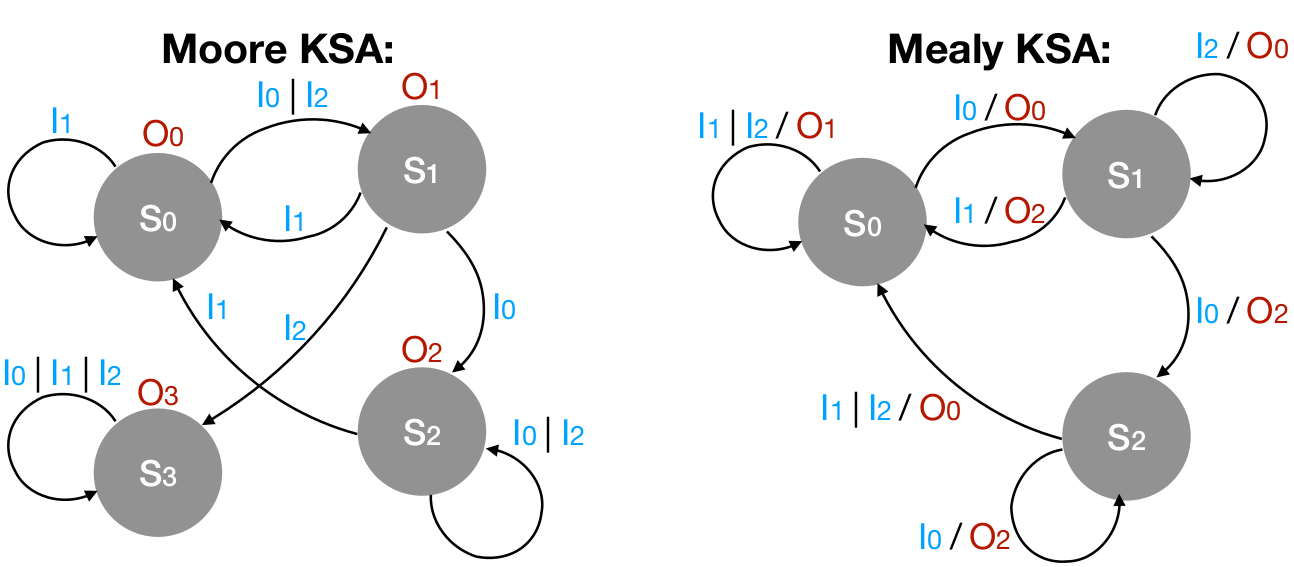
\includegraphics[scale = 0.3]{img/Diagram.png}
\end{figure}

\subsubsection{Pomocí soustavy rovnic}
Vlevo tvar rovnic pro Mooreův automat, vpravo pro Mealyho automat:\\
\begin{figure}[h!]
    \centering
    \begin{minipage}[b]{0.4\textwidth}
        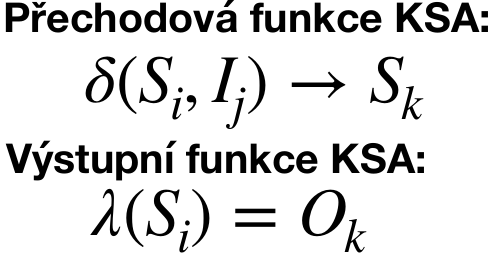
\includegraphics[width=\textwidth]{img/MooreSoustava.png}
    \end{minipage}
    \hfill
    \begin{minipage}[b]{0.4\textwidth}
        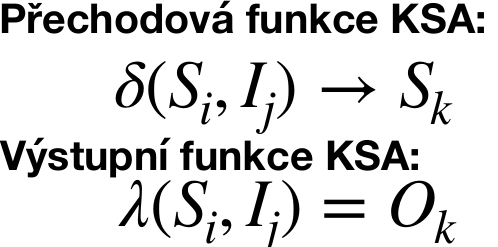
\includegraphics[width=\textwidth]{img/MealySoustava.png}
    \end{minipage}
\end{figure}

\begin{figure}[h!]
    \centering
    \begin{minipage}[b]{0.4\textwidth}
        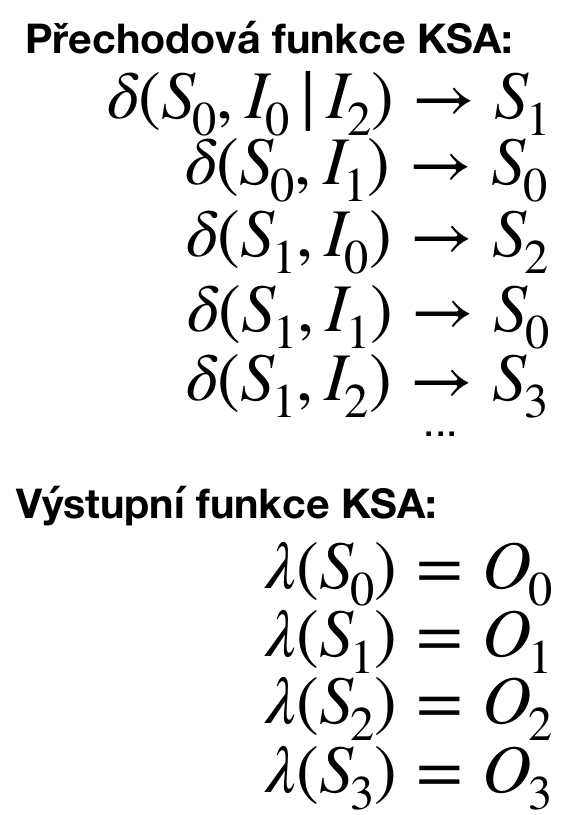
\includegraphics[width=\textwidth]{img/MooreRovnice.png}
    \end{minipage}
    \hfill
    \begin{minipage}[b]{0.4\textwidth}
        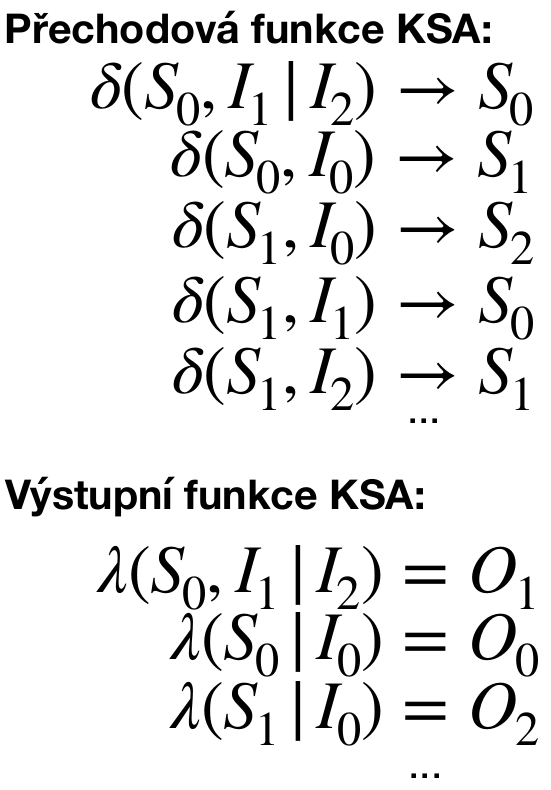
\includegraphics[width=\textwidth]{img/MealyRovnice.png}
    \end{minipage}
\end{figure}

\subsubsection{Pomocí tabulek}
Opět vlevo Moore, vpravo Mealy:\\
\begin{figure}[h!]
    \centering
    \begin{minipage}[b]{0.4\textwidth}
        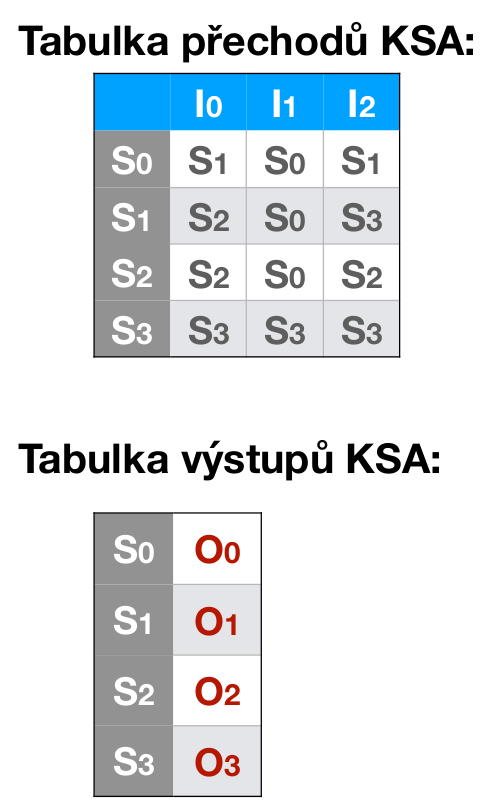
\includegraphics[scale = 0.2]{img/MooreTabulky.png}
    \end{minipage}
    \hfill
    \begin{minipage}[b]{0.4\textwidth}
        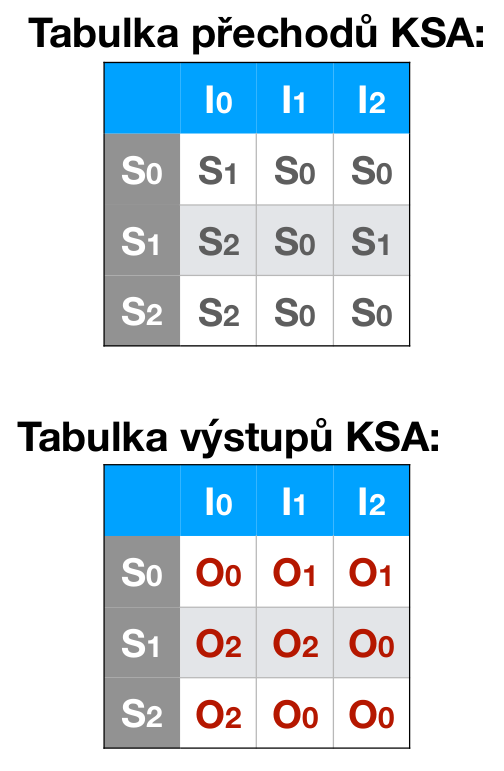
\includegraphics[scale = 0.2]{img/Mealy tabulky.png}
    \end{minipage}
\end{figure}

\subsection{Autonomní automat}
Systém bez vstupů, mimo hodinového.\\
Následující stav je odvozen pouze ze stavu současného: \(Q^{t+1} = \delta(Q^t)\).\\
Např. jednoduché čítače jsou autonomní automaty.\\